\documentclass[11pt,a4paper]{article}
\usepackage[top=3cm,bottom=3cm,left=4cm,right=3cm]{geometry}
\usepackage[T1]{fontenc}
\usepackage{lmodern}
\usepackage{microtype}
\usepackage{amsmath}
\usepackage{amssymb}
\usepackage{xurl}
\usepackage{graphicx}
\usepackage{caption}
\usepackage{float}
\usepackage{array}
\usepackage{tabularx}
\usepackage{enumitem}
\usepackage{xcolor}
\usepackage{tikz}
\usepackage{listings}
\usepackage{fancyhdr}
\usepackage[colorlinks=true,linkcolor=blue,urlcolor=blue]{hyperref}

% ---------------------------------------------------------------------------
% Istilah dalam Bahasa Indonesia (tanpa babel agar kompatibel di semua TeX)
% ---------------------------------------------------------------------------
\renewcommand{\contentsname}{Daftar Isi}
\renewcommand{\figurename}{Gambar}
\renewcommand{\tablename}{Tabel}
\renewcommand{\lstlistingname}{Kode}
\renewcommand{\appendixname}{Lampiran}

% ---------------------------------------------------------------------------
% Header dan footer
% ---------------------------------------------------------------------------
\pagestyle{fancy}
\fancyhf{}
\fancyhead[L]{Modul 0 -- Pengenalan Kit Praktikum}
\fancyhead[R]{\nouppercase{\leftmark}}
\fancyfoot[L]{TF4015 Sistem Kontrol Diskrit}
\fancyfoot[R]{\thepage}
\renewcommand{\footrulewidth}{0.4pt}
\setlength{\headheight}{14pt}

% ---------------------------------------------------------------------------
% Gaya penulisan kode Arduino
% ---------------------------------------------------------------------------
\lstset{
	language=C++,
	basicstyle=\ttfamily\footnotesize,
	keywordstyle=\color{blue!70!black}\bfseries,
	commentstyle=\color{green!45!black},
	stringstyle=\color{red!65!black},
	numbers=left,
	numberstyle=\tiny\color{gray},
	frame=single,
	breaklines=true,
	tabsize=2,
	showstringspaces=false,
	columns=fullflexible,
	keepspaces=true,
	morekeywords={byte,uint32_t,String}
}

% ---------------------------------------------------------------------------
% Makro bantu
% ---------------------------------------------------------------------------
% Nama sketch utama program praktikum. Ubah di sini bila nama di repositori berbeda.
\newcommand{\sketch}{\texttt{SKD23.ino}}
% Nama file/program dalam teks
\newcommand{\prog}[1]{\texttt{#1}}
% Gambar dengan placeholder: bila file belum ada, ditampilkan kotak penanda
\newcommand{\gambar}[4]{%
	\begin{figure}[H]
		\centering
		\IfFileExists{#1}{%
			\includegraphics[width=#2]{#1}%
		}{%
			\fbox{\parbox[c][4cm][c]{0.7\textwidth}{\centering\small\textcolor{red}{Gambar belum tersedia:}\\\texttt{\detokenize{#1}}}}%
		}
		\caption{#3}
		\label{#4}
	\end{figure}}
% Kotak catatan / peringatan
\newcommand{\peringatan}[1]{%
	\begin{center}
		\fcolorbox{red!70!black}{red!5}{\parbox{0.92\textwidth}{\textbf{Peringatan.} #1}}
	\end{center}}
\newcommand{\catatan}[1]{%
	\begin{center}
		\fcolorbox{blue!60!black}{blue!4}{\parbox{0.92\textwidth}{\textbf{Catatan.} #1}}
	\end{center}}

\newcolumntype{C}{>{\centering\arraybackslash}X}
\setlist[itemize]{itemsep=2pt,topsep=4pt}
\setlist[enumerate]{itemsep=2pt,topsep=4pt}

\begin{document}

% ===========================================================================
% Halaman judul
% ===========================================================================
\begin{titlepage}
	\centering
	\vspace*{2cm}
	{\large TF4015 -- Sistem Kontrol Diskrit\par}
	\vspace{2.5cm}
	{\Large Praktikum\par}
	\vspace{0.4cm}
	{\huge\bfseries Modul 0\par}
	\vspace{0.4cm}
	{\LARGE Pengenalan Kit Praktikum\\Sistem Kontrol Diskrit\par}
	\vfill
	% TODO: sesuaikan nama tim pengajar dan asisten
	{\large Tim Pengajar TF4015\par}
	\vspace{0.3cm}
	{\large Program Studi Teknik Fisika\\Fakultas Teknologi Industri\\Institut Teknologi Bandung\par}
	\vspace{0.8cm}
	{\large Semester I 2026/2027\par}
\end{titlepage}

\pagenumbering{roman}
\tableofcontents
\newpage
\pagenumbering{arabic}
\setcounter{page}{1}

% ===========================================================================
\section{Pendahuluan}
% ===========================================================================
\subsection{Latar Belakang}
Sistem Kontrol Diskrit (SKD) merupakan salah satu cabang penting dalam teknik kendali yang mempelajari analisis dan perancangan sistem kontrol dengan sinyal yang bernilai diskrit terhadap waktu. Berbeda dengan sistem kontrol analog konvensional, implementasi kontrol diskrit modern memanfaatkan perangkat komputasi digital, seperti mikrokontroler, PLC, atau komputer, sebagai pengendali utama. Pengendali digital hanya dapat ``melihat'' sistem fisik pada saat-saat pencacahan (\textit{sampling}) dan hanya dapat memberikan aksi kontrol melalui konverter, sehingga pemahaman tentang perangkat keras dan pewaktuan menjadi bagian yang tidak terpisahkan dari perancangan kontrol diskrit.

Praktikum Sistem Kontrol Diskrit (\textbf{TF4015}) dirancang untuk memberikan pengalaman praktis dan aplikatif tentang pengontrolan nyata kepada mahasiswa. Melalui praktikum ini, praktikan akan dibimbing secara sistematis, mulai dari mengenali komponen fisik, mengidentifikasi karakteristik sistem seperti \textit{deadzone} dan dinamika motor, hingga merancang, menyimulasikan, menerapkan, serta menala algoritma kontrol kalang tertutup (\textit{closed-loop control}).

Sebelum masuk ke modul identifikasi sistem dan modul-modul kontrol, \textbf{Modul 0 -- Pengenalan Kit Praktikum} ini menjadi fondasi yang krusial. Modul ini menjembatani pemahaman praktikan terhadap kit praktikum SKD yang akan digunakan secara intensif sepanjang semester. Kit praktikum ini mengintegrasikan tiga subsistem utama sistem kontrol:

\begin{enumerate}
	\item \textbf{Sistem (\textit{plant})}: motor DC sebagai aktuator yang dikendalikan, dilengkapi tachometer (sensor kecepatan) dan potensiometer (sensor posisi).
	\item \textbf{Kontroler}: Arduino UNO dan PCB \textit{shield} yang berisi rangkaian driver motor serta pengkondisi sinyal sensor.
	\item \textbf{Catu daya (\textit{power supply})}: penyedia tegangan 24~V untuk motor dan 5~V untuk rangkaian elektronik.
\end{enumerate}

Pemahaman awal mengenai fungsi dan batas operasional setiap komponen, pemetaan pin antarmuka, struktur program, serta prosedur pengoperasian yang aman sangat penting, baik untuk kelancaran praktikum maupun untuk menjaga kit praktikum tetap dalam kondisi baik.

\subsection{Tujuan Praktikum}
Setelah menyelesaikan seluruh kegiatan pada Modul 0, praktikan diharapkan mampu:

\begin{enumerate}
	\item Mengidentifikasi subsistem utama kit praktikum SKD (sistem, kontroler, dan catu daya) beserta level tegangan kerjanya (24~V dan 5~V).
	\item Menjelaskan spesifikasi dan prinsip kerja komponen utama kit, yaitu motor DC COPAL LC32F-184VF, tachometer, potensiometer OVTER WDD35D4, Arduino UNO, serta rangkaian driver motor dan pengkondisi sinyal pada PCB.
	\item Menyiapkan perangkat lunak praktikum (Arduino IDE beserta \textit{library}, MATLAB) dan memahami struktur program praktikum.
	\item Menerapkan prosedur keselamatan kerja dan prosedur standar operasional (SOP) untuk mencegah kerusakan kit praktikum.
	\item Melakukan akuisisi data sensor dan menampilkannya melalui \textit{Serial Monitor} dan \textit{Serial Plotter}.
	\item Membedakan pewaktuan program menggunakan \texttt{delay()} dan pewaktuan berbasis waktu cacah (\textit{time sampling}).
	\item Menggerakkan motor ke dua arah putar melalui masukan serial dan mengamati respons kedua sensor.
\end{enumerate}

\subsection{Peralatan dan Perangkat Lunak}
Peralatan yang digunakan pada Modul 0 ditunjukkan pada Tabel~\ref{tab:peralatan_praktikum}.

\begin{table}[H]
	\centering
	\caption{Daftar peralatan praktikum Modul 0}
	\label{tab:peralatan_praktikum}
	\begin{tabularx}{\textwidth}{|c|X|c|l|}
		\hline
		\textbf{No} & \textbf{Nama Peralatan}                  & \textbf{Jumlah} & \textbf{Keterangan}          \\
		\hline
		1           & Kit Praktikum SKD                        & 1               & Disediakan asisten           \\
		2           & Kabel USB tipe A--B                      & 1               & Disediakan bersama kit       \\
		3           & Multimeter (AVO meter)                   & 1               & Disediakan asisten           \\
		4           & Laptop                                   & 1               & Milik praktikan              \\
		5           & Arduino IDE + library Adafruit MCP4725   & 1               & Terinstal pada laptop        \\
		6           & MATLAB (desktop atau MATLAB Online)      & 1               & Terinstal / akun aktif       \\
		7           & Perangkat lunak \textit{spreadsheet}     & 1               & Excel, Google Sheets, dll.   \\
		8           & Program praktikum                        & 1               & Unduh dari repositori        \\
		\hline
	\end{tabularx}
\end{table}

Tautan perangkat lunak:
\begin{itemize}
	\item Arduino IDE: \url{https://www.arduino.cc/en/software}
	\item MATLAB Online: \url{https://matlab.mathworks.com}
	\item Program praktikum: \url{https://github.com/faqihza/TF4015---Sistem-Kontrol-Diskrit}
\end{itemize}

\subsection{Peta Praktikum}
Modul 0 merupakan bagian pertama dari rangkaian praktikum SKD. Seluruh modul menggunakan kit praktikum yang sama dan saling berkesinambungan, seperti ditunjukkan pada Tabel~\ref{tab:peta_praktikum}. Keluaran setiap modul menjadi masukan bagi modul berikutnya, sehingga kit yang sama sebaiknya digunakan oleh kelompok yang sama hingga akhir praktikum.

\begin{table}[H]
	\centering
	\caption{Rangkaian modul praktikum Sistem Kontrol Diskrit}
	\label{tab:peta_praktikum}
	\begin{tabularx}{\textwidth}{|c|l|X|}
		\hline
		\textbf{Modul} & \textbf{Judul}           & \textbf{Keluaran utama}                                                        \\
		\hline
		0              & Pengenalan Kit Praktikum & Kit dan perangkat lunak siap, praktikan memahami komponen, program, dan SOP     \\
		1              & Identifikasi Sistem      & Kompensasi \textit{deadzone}, waktu cacah, dan model kecepatan motor DC          \\
		2              & Kontrol Kecepatan        & Pengontrol P/PI/PID kecepatan hasil penalaan dan penalaan halus                  \\
		3              & Kontrol Posisi           & Model posisi dan pengontrol posisi yang diuji terhadap gangguan                  \\
		4              & \textit{Pole Placement} dan Observer & Pengontrol umpan balik keadaan dengan penempatan kutub serta observer posisi dan kecepatan \\
		\hline
	\end{tabularx}
\end{table}

% ===========================================================================
\section{Teori Dasar}
% ===========================================================================
\subsection{Arsitektur Kit Praktikum}
Kit praktikum SKD dirancang sebagai representasi fisik dari sistem kontrol digital kalang tertutup. Foto kit praktikum ditunjukkan pada Gambar~\ref{fig:kit_praktikum}, sedangkan arsitekturnya ditunjukkan pada Gambar~\ref{fig:skd_arsitektur}. Secara umum, kit dibagi menjadi tiga subsistem:

\gambar{assets/kit_praktikum.jpg}{0.85\textwidth}{Kit praktikum Sistem Kontrol Diskrit}{fig:kit_praktikum}

\begin{enumerate}
	\item \textbf{Sistem (motor dan sensor)}: objek fisik yang dikendalikan, yaitu motor DC, beserta sensor yang mengukur keluarannya, yaitu potensiometer untuk posisi dan tachometer untuk kecepatan.
	\item \textbf{Kontroler (Arduino UNO dan PCB \textit{shield})}: Arduino UNO menjalankan program akuisisi data dan algoritma kontrol diskrit. PCB \textit{shield} kustom dipasang di atas Arduino UNO dan berisi rangkaian driver motor, rangkaian pengkondisi sinyal sensor, serta konektor yang menghubungkan seluruh komponen kit.
	\item \textbf{Catu daya}: penyedia daya listrik DC yang stabil untuk menggerakkan motor (24~V) serta menghidupkan komponen elektronik pada PCB (5~V).
\end{enumerate}

\gambar{assets/skd_arsitektur.png}{0.9\textwidth}{Arsitektur kit praktikum Sistem Kontrol Diskrit}{fig:skd_arsitektur}

Hubungan ketiga subsistem pada Gambar~\ref{fig:skd_arsitektur} merupakan struktur sistem kontrol digital yang umum. Kontroler digital berinteraksi dengan dunia fisik yang bersifat kontinu melalui dua antarmuka: \textit{Analog-to-Digital Converter} (ADC) untuk membaca sensor dan \textit{Digital-to-Analog Converter} (DAC) untuk memberikan aksi kontrol kepada aktuator.

\subsection{Spesifikasi dan Karakteristik Komponen}

\subsubsection{Aktuator: Motor DC COPAL LC32F-184VF}
Motor yang digunakan adalah motor DC COPAL tipe LC32F-184VF (Gambar~\ref{fig:motor_dc}), yaitu motor DC berkomutator sikat (\textit{brushed DC motor}). Pada bagian belakang motor terpasang tachometer yang porosnya menyatu dengan poros motor. Spesifikasi motor ditunjukkan pada Tabel~\ref{tab:spek_motor}.

\gambar{assets/motor_DC.png}{0.3\textwidth}{Motor DC COPAL LC32F-184VF}{fig:motor_dc}

% TODO: verifikasi nilai berikut terhadap datasheet COPAL LC32F-184VF.
% Arus awal (starting current) seharusnya lebih besar dari arus nominal; nilai 160 mA
% kemungkinan adalah arus tanpa beban (no-load current).
\begin{table}[H]
	\centering
	\caption{Spesifikasi motor DC COPAL LC32F-184VF}
	\label{tab:spek_motor}
	\begin{tabular}{|l|r|}
		\hline
		\textbf{Parameter}             & \textbf{Nilai} \\
		\hline
		Tegangan kerja                 & 24 V DC        \\
		Arus nominal (\textit{rated})  & 1,2 A          \\
		Arus maksimum                  & 2,4 A          \\
		Torsi nominal                  & 16,1 mNm       \\
		Torsi maksimum                 & 48 mNm         \\
		Kecepatan nominal              & 6400 rpm       \\
		Kecepatan tanpa beban          & 8230 rpm       \\
		Torsi awal                     & 21 mNm         \\
		Arus tanpa beban               & 160 mA         \\
		\hline
	\end{tabular}
\end{table}

Motor diputar dengan memberikan beda tegangan pada kedua terminalnya (kabel merah dan kabel putih). Arah putar ditentukan oleh polaritas tegangan: membalik polaritas akan membalik arah putar. Pada kit ini, pengaturan polaritas dilakukan oleh IC driver L293D (Bagian~\ref{sec:driver_motor}), sedangkan besar tegangan menentukan torsi dan kecepatan putar motor.

\subsubsection{Sensor Kecepatan: Tachometer}
Tachometer (Gambar~\ref{fig:tachometer}) terpasang menyatu dengan bagian belakang motor DC untuk mengukur kecepatan putar.
\begin{itemize}
	\item \textbf{Tipe}: sensor kontak dan analog yang bekerja berdasarkan induksi magnetik.
	\item \textbf{Prinsip kerja}: poros tachometer terhubung langsung dengan poros motor. Ketika motor berputar, magnet pada poros tachometer ikut berputar dan menginduksi tegangan bolak-balik berbentuk sinusoidal pada kumparan tachometer. Sinyal keluaran dikirimkan melalui kabel berwarna hijau.
	\item \textbf{Karakteristik}: amplitudo (dan frekuensi) sinyal keluaran bertambah seiring bertambahnya kecepatan putar motor. Karena sinyalnya bolak-balik, sinyal ini perlu disearahkan dan difilter sebelum dapat dibaca oleh ADC Arduino (Bagian~\ref{sec:pengkondisi_kecepatan}).
\end{itemize}

\gambar{assets/tachometer.png}{0.3\textwidth}{Tachometer yang terpasang pada motor DC}{fig:tachometer}

\subsubsection{Sensor Posisi: Potensiometer OVTER WDD35D4}
Potensiometer putar (\textit{rotary}) tipe WDD35D4 (Gambar~\ref{fig:potensiometer}) digunakan sebagai sensor posisi sudut. Karakteristiknya adalah sebagai berikut:

\gambar{assets/potensiometer.png}{0.3\textwidth}{Potensiometer OVTER WDD35D4}{fig:potensiometer}

\begin{itemize}
	\item \textbf{Hambatan}: $10~\mathrm{k\Omega} \pm 15\%$.
	\item \textbf{Linearitas independen}: $0{,}5\%$, artinya penyimpangan hubungan sudut mekanis terhadap tegangan keluaran dari garis lurus tidak lebih dari $0{,}5\%$ rentang penuh.
	\item \textbf{Sistem roda gigi}: potensiometer tidak terhubung langsung ke poros motor, melainkan digerakkan melalui sepasang roda gigi akrilik. Perbandingan jumlah gigi roda gigi motor terhadap roda gigi potensiometer adalah $16:100$. Dengan asumsi tidak ada slip, hubungan sudut putar motor $\theta_m$ dan sudut putar potensiometer $\theta_p$ adalah
	      \begin{equation}
		      \theta_p = \frac{16}{100}\,\theta_m ,
		      \label{eq:rasio_gigi}
	      \end{equation}
	      sehingga satu putaran penuh potensiometer setara dengan $6{,}25$ putaran motor.
	\item \textbf{Pin}:
	      \begin{itemize}
		      \item Pin 1: \textit{ground} (GND)
		      \item Pin 2: sinyal tegangan keluaran ($V_{out}$)
		      \item Pin 3: tegangan referensi ($V_{ref}$)
	      \end{itemize}
\end{itemize}

\subsubsection{Unit Pemroses: Arduino UNO}
Arduino UNO (Gambar~\ref{fig:arduino_uno}) berfungsi sebagai kontroler digital. Mikrokontroler ATmega328P dengan \textit{clock} 16~MHz pada Arduino UNO menjalankan pembacaan sensor, perhitungan algoritma kontrol, dan pengiriman perintah ke driver motor. PCB \textit{shield} kit praktikum dipasang di atas Arduino UNO sehingga pin-pin Arduino langsung terhubung ke rangkaian pada PCB.

\gambar{assets/arduino_uno.jpg}{0.6\textwidth}{Arduino UNO}{fig:arduino_uno}

\begin{itemize}
	\item \textbf{Masukan analog}: 6 pin (A0--A5) yang terhubung ke ADC internal 10-bit. ADC mengubah tegangan $0$--$5$~V menjadi bilangan bulat $0$--$1023$.
	\item \textbf{Digital I/O}: 14 pin (D0--D13) untuk sinyal logika HIGH/LOW. Pada kit ini, pin D9--D11 digunakan untuk mengatur arah putar motor melalui L293D.
	\item \textbf{Komunikasi I$^2$C}: pin SDA (A4) dan SCL (A5) digunakan untuk mengirim perintah digital ke DAC eksternal MCP4725.
	\item \textbf{Komunikasi serial (USB)}: digunakan untuk mengunggah program serta mengirim dan menerima data dari laptop melalui \textit{Serial Monitor}. Pin D0 (RX) dan D1 (TX) dipakai oleh jalur ini sehingga tidak digunakan untuk keperluan lain.
\end{itemize}

Pemetaan pin Arduino UNO pada kit praktikum dirangkum pada Tabel~\ref{tab:pin_arduino}.

\begin{table}[H]
	\centering
	\caption{Pemetaan pin Arduino UNO pada kit praktikum}
	\label{tab:pin_arduino}
	\begin{tabularx}{\textwidth}{|c|l|X|X|}
		\hline
		\textbf{Pin} & \textbf{Nama di program}          & \textbf{Terhubung ke}  & \textbf{Fungsi}                                \\
		\hline
		A0           & \texttt{PinTachometer}            & Pengkondisi sinyal tachometer & Membaca kecepatan putar motor            \\
		A1           & \texttt{PinPotensiometer}         & Pengkondisi sinyal potensiometer & Membaca posisi sudut                  \\
		A4 (SDA)     & --                                & MCP4725                & Data I$^2$C ke DAC (alamat \texttt{0x60})      \\
		A5 (SCL)     & --                                & MCP4725                & \textit{Clock} I$^2$C ke DAC                   \\
		D11          & \texttt{PinEn}                    & L293D (3-4EN)          & Mengaktifkan kanal driver motor                \\
		D10          & \texttt{PinIn1}                   & L293D (masukan arah)   & HIGH saat masukan motor positif                \\
		D9           & \texttt{PinIn2}                   & L293D (masukan arah)   & HIGH saat masukan motor negatif                \\
		D0, D1       & --                                & USB (serial)           & Komunikasi dengan laptop                       \\
		\hline
	\end{tabularx}
\end{table}

\subsubsection{Catu Daya}
Kit praktikum menggunakan dua level tegangan:
\begin{itemize}
	\item \textbf{Power supply AC--DC 24~V} (Gambar~\ref{fig:power_supply}): mengubah tegangan jala-jala 220~V AC menjadi 24~V DC dengan arus keluaran maksimum 1,5~A. Tegangan ini dipakai untuk menggerakkan motor melalui rangkaian driver.
	\item \textbf{Konverter DC--DC 5~V} (Gambar~\ref{fig:dc_to_dc}): menurunkan tegangan 24~V menjadi 5~V (dapat diatur melalui trimpot pada modul). Konverter ini menjadi suplai tambahan bagi IC pada PCB bila daya dari Arduino UNO (yang ditenagai port USB laptop) tidak mencukupi.
\end{itemize}

\begin{figure}[H]
	\centering
	\begin{minipage}{0.48\textwidth}
		\centering
		\IfFileExists{assets/power_supply.jpg}{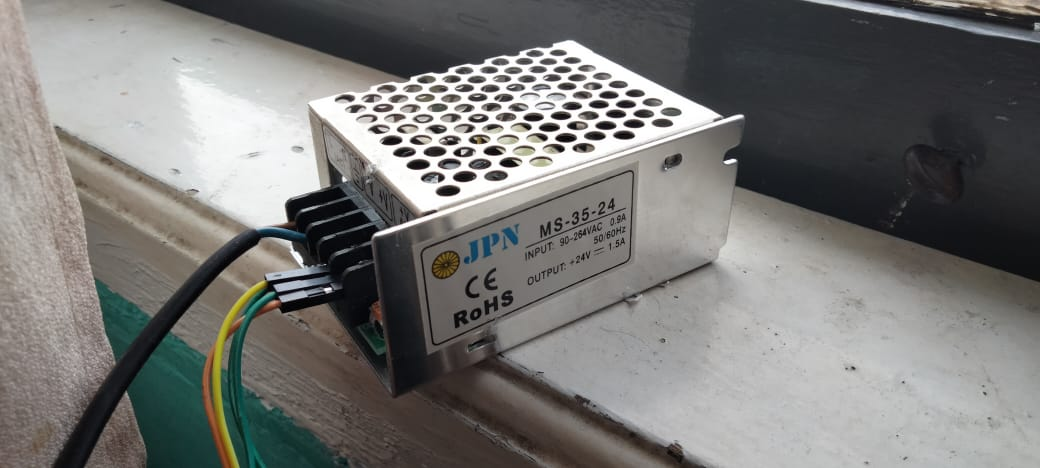
\includegraphics[width=\textwidth]{assets/power_supply.jpg}}{\fbox{assets/power\_supply.jpg}}
		\caption{Power supply 24~V}
		\label{fig:power_supply}
	\end{minipage}\hfill
	\begin{minipage}{0.48\textwidth}
		\centering
		\IfFileExists{assets/dc_to_dc.jpg}{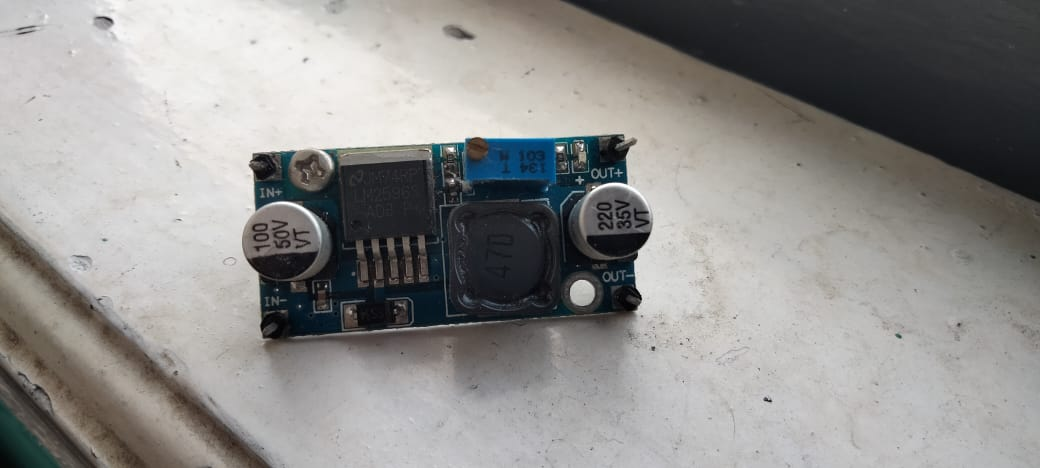
\includegraphics[width=\textwidth]{assets/dc_to_dc.jpg}}{\fbox{assets/dc\_to\_dc.jpg}}
		\caption{Konverter DC--DC}
		\label{fig:dc_to_dc}
	\end{minipage}
\end{figure}

\catatan{Perhatikan bahwa arus maksimum power supply (1,5~A) lebih kecil daripada arus maksimum motor (2,4~A). Menahan poros motor yang sedang diberi masukan besar akan membebani power supply, driver, dan transistor secara berlebihan.}

\subsection{Rangkaian PCB Kit Praktikum}
Seluruh rangkaian elektronik kit praktikum diintegrasikan pada satu PCB \textit{shield} kustom (Gambar~\ref{fig:pcb_shield}) yang terdiri atas tiga rangkaian utama:
\begin{enumerate}
	\item rangkaian driver motor,
	\item rangkaian pengkondisi sinyal sensor kecepatan, dan
	\item rangkaian pengkondisi sinyal sensor posisi.
\end{enumerate}

\begin{figure}[H]
	\centering
	\begin{minipage}{0.48\textwidth}
		\centering
		\IfFileExists{assets/pcb_shield.jpg}{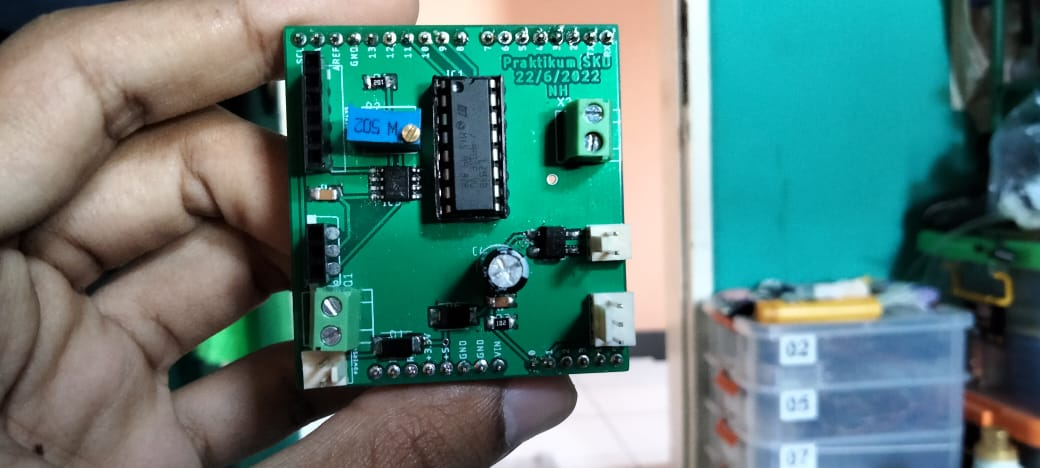
\includegraphics[width=\textwidth]{assets/pcb_shield.jpg}}{\fbox{assets/pcb\_shield.jpg}}
	\end{minipage}\hfill
	\begin{minipage}{0.48\textwidth}
		\centering
		\IfFileExists{assets/shield_terpasang.jpg}{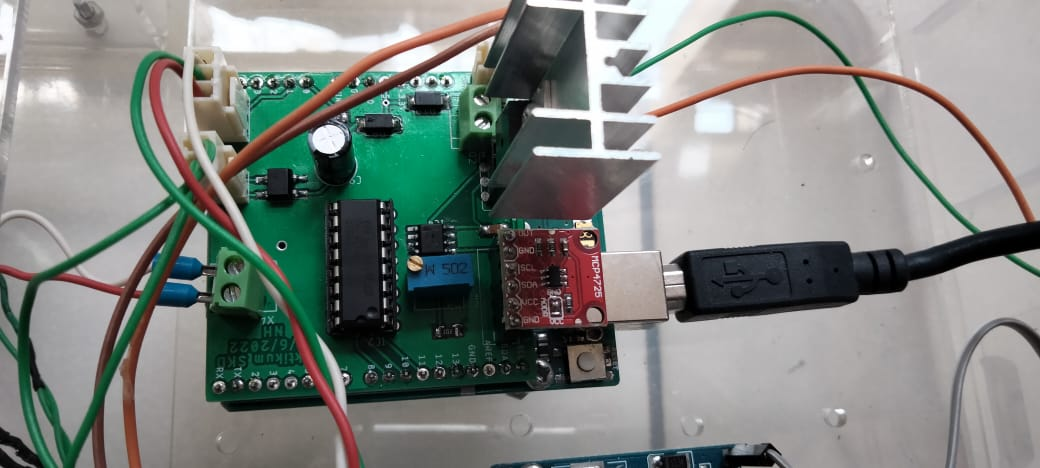
\includegraphics[width=\textwidth]{assets/shield_terpasang.jpg}}{\fbox{assets/shield\_terpasang.jpg}}
	\end{minipage}
	\caption{PCB \textit{shield} kit praktikum sebelum dipasang (kiri) dan setelah terpasang pada Arduino UNO beserta konektornya (kanan)}
	\label{fig:pcb_shield}
\end{figure}

\subsubsection{Rangkaian Driver Motor}
\label{sec:driver_motor}
Rangkaian driver motor (Gambar~\ref{fig:driver_motor}) dirancang agar Arduino UNO dapat mengatur besar tegangan motor (yang menentukan kecepatan) sekaligus arah putarnya. Rantai sinyal pada rangkaian ini adalah:
\begin{center}
	Arduino $\xrightarrow{\text{I}^2\text{C}}$ DAC MCP4725 $\xrightarrow{0\text{--}5\,\text{V}}$ OpAmp AD712 $\rightarrow$ Transistor TIP41C $\xrightarrow{V_{CC2}}$ L293D $\rightarrow$ Motor
\end{center}

\gambar{assets/driver_motor.png}{0.95\textwidth}{Skematik rangkaian driver motor}{fig:driver_motor}

\paragraph{DAC MCP4725.}
\begin{itemize}
	\item Arduino UNO tidak memiliki DAC internal; pin PWM Arduino hanya menghasilkan sinyal digital yang dimodulasi lebar pulsanya. Oleh karena itu digunakan DAC eksternal MCP4725.
	\item MCP4725 adalah DAC 12-bit yang berkomunikasi dengan Arduino melalui I$^2$C (pin SDA dan SCL). Nilai digital $0$--$4095$ diubah menjadi tegangan analog $0$--$5$~V pada pin OUT.
\end{itemize}

\paragraph{\textit{Operational amplifier} AD712.}
\begin{itemize}
	\item Tegangan keluaran DAC maksimum 5~V, sedangkan motor membutuhkan hingga 24~V. Tegangan DAC dikuatkan menggunakan OpAmp AD712 yang disuplai 24~V.
	\item OpAmp disusun sebagai penguat \textit{non-inverting} dengan penguatan
	      \begin{equation}
		      A_v = 1 + \frac{R_2}{R_1},
		      \label{eq:penguatan_opamp}
	      \end{equation}
	      dengan $R_1 = 1~\mathrm{k\Omega}$ dan $R_2$ berupa trimpot $5~\mathrm{k\Omega}$. Dengan memutar trimpot, penguatan dapat diatur secara manual. Pengaturan trimpot ini akan dibahas pada Modul 1; \textbf{jangan mengubah posisi trimpot pada Modul 0}.
\end{itemize}

\paragraph{Transistor TIP41C.}
\begin{itemize}
	\item OpAmp hanya mampu mengalirkan arus yang kecil. Bila keluaran OpAmp langsung dihubungkan ke motor, tegangan akan turun dan motor berputar lambat.
	\item Transistor TIP41C dipasang sebagai penguat arus (\textit{emitter follower}): kolektor terhubung ke suplai 24~V, basis menerima keluaran OpAmp, dan emitor menyuplai pin $V_{CC2}$ pada L293D. Tegangan emitor kurang lebih sama dengan tegangan basis dikurangi tegangan basis--emitor (sekitar 0,7~V), tetapi dengan kemampuan arus yang jauh lebih besar.
	\item Transistor dilengkapi \textit{heat sink} untuk membuang panas akibat daya yang terdisipasi.
\end{itemize}

\paragraph{\textit{Half-H driver} L293D.}
\begin{itemize}
	\item L293D berisi rangkaian \textit{H-bridge} yang menghubungkan kedua terminal motor ke $V_{CC2}$ atau GND sehingga polaritas tegangan motor, dan dengan demikian arah putarnya, dapat dibalik.
	\item L293D mendapatkan \textbf{daya motor} dari transistor TIP41C melalui pin $V_{CC2}$, sedangkan \textbf{sinyal logika arah} diterima langsung dari pin digital Arduino.
	\item Kombinasi logika pin pengendali L293D dan aksi yang dihasilkan ditunjukkan pada Tabel~\ref{tab:logika_l293d}. Pada program praktikum, kombinasi ini diatur oleh fungsi \texttt{clock\_wise()}, \texttt{counter\_clock\_wise()}, dan \texttt{fast\_break()}.
	\item Dioda proteksi dan kapasitor \textit{bypass} pada rangkaian berfungsi meredam tegangan balik (\textit{back-EMF}) induktif dari motor dan derau suplai.
\end{itemize}

\begin{table}[htbp]
	\centering
	\caption{Logika pengendalian arah motor oleh L293D pada program praktikum}
	\label{tab:logika_l293d}
	\begin{tabularx}{\textwidth}{|C|C|C|X|l|}
		\hline
		\textbf{EN (D11)} & \textbf{IN1 (D10)} & \textbf{IN2 (D9)} & \textbf{Kondisi motor} & \textbf{Fungsi program} \\
		\hline
		LOW               & x                  & x                 & Terputus (mengambang)  & --                       \\
		HIGH              & HIGH               & LOW               & Berputar arah positif  & \texttt{clock\_wise()}         \\
		HIGH              & LOW                & HIGH              & Berputar arah negatif  & \texttt{counter\_clock\_wise()} \\
		HIGH              & LOW                & LOW               & Direm (kedua terminal ke GND) & \texttt{fast\_break()}  \\
		\hline
	\end{tabularx}
\end{table}

\catatan{Nama fungsi \texttt{clock\_wise()} hanya penamaan di program. Arah putar fisik yang sebenarnya (searah atau berlawanan jarum jam) bergantung pada pemasangan kabel motor dan akan diverifikasi pada Percobaan~5.}

Dengan masukan motor $u$ dalam persen ($-100 \le u \le 100$), program mengirim nilai digital ke DAC sebesar
\begin{equation}
	N_{DAC} = \frac{4095\,|u|}{100},
	\qquad
	V_{DAC} = \frac{5\,|u|}{100}~\text{V},
	\label{eq:dac}
\end{equation}
sedangkan tanda $u$ menentukan arah putar melalui L293D. Tegangan motor kemudian kurang lebih sebesar $A_v V_{DAC}$ dikurangi rugi tegangan pada transistor dan L293D, dengan batas atas mendekati tegangan suplai 24~V.

\subsubsection{Rangkaian Pengkondisi Sinyal Sensor Kecepatan}
\label{sec:pengkondisi_kecepatan}
Sinyal tachometer berupa tegangan bolak-balik sehingga tidak dapat langsung dibaca oleh ADC Arduino yang hanya menerima tegangan $0$--$5$~V. Rangkaian pengkondisi sinyal kecepatan (Gambar~\ref{fig:rangkaian_tacho}) terdiri atas:
\begin{enumerate}
	\item \textbf{Penyearah gelombang penuh} (\textit{bridge rectifier}) MB6S (BR1), yang mengubah sinyal sinusoidal dari konektor TACHO menjadi sinyal searah (selalu positif).
	\item \textbf{Filter kapasitor}, berupa kapasitor elektrolit C4 ($100~\mu\mathrm{F}$) dan kapasitor keramik C2 ($100~\mathrm{nF}$) yang dipasang paralel terhadap keluaran penyearah. C4 meratakan riak (\textit{ripple}) hasil penyearahan, sedangkan C2 meredam derau frekuensi tinggi.
	\item \textbf{Resistor beban} R3 ($1~\mathrm{k\Omega}$) yang dipasang paralel dengan kapasitor sebagai jalur pengosongan muatan. Tanpa R3, kapasitor akan tetap bermuatan ketika motor melambat sehingga tegangan pada pin A0 tidak mengikuti penurunan kecepatan.
	\item \textbf{Dioda Schottky} D6 (SS32) yang menghubungkan keluaran ke jalur 5~V Arduino. Dioda ini menjadi penjepit (\textit{clamp}): bila tegangan tachometer pada kecepatan tinggi melebihi 5~V, kelebihan tegangan dialirkan ke jalur 5~V sehingga pin ADC terlindungi.
\end{enumerate}
Keluaran rangkaian ini dihubungkan ke pin A0 Arduino UNO dan tegangannya sebanding dengan kecepatan putar motor.

Perlu diperhatikan bahwa filter ini juga memengaruhi dinamika pengukuran. Ketika kecepatan motor turun, tegangan pada C4 berkurang melalui R3 dengan konstanta waktu
\begin{equation}
	\tau_f = R_3\,C_4 = (1~\mathrm{k\Omega})(100~\mu\mathrm{F}) = 0{,}1~\text{s}.
	\label{eq:tau_filter}
\end{equation}
Sebaliknya, ketika kecepatan naik, kapasitor diisi melalui penyearah dengan hambatan yang jauh lebih kecil sehingga pengisiannya berlangsung lebih cepat. Akibatnya, bacaan kecepatan dapat merespons kenaikan dan penurunan kecepatan dengan laju yang berbeda.

\gambar{assets/rangkaian_tachometer.png}{0.75\textwidth}{Skematik rangkaian pengkondisi sinyal sensor kecepatan}{fig:rangkaian_tacho}

\subsubsection{Rangkaian Pengkondisi Sinyal Sensor Posisi}
\label{sec:pengkondisi_posisi}
Rangkaian sensor posisi (Gambar~\ref{fig:rangkaian_poten}) berupa rangkaian pembagi tegangan. Pin 3 potensiometer dihubungkan ke jalur 5~V Arduino ($V_{ref} = 5$~V) dan pin 1 ke GND, sehingga tegangan pada pin \textit{wiper} (pin 2) sebanding dengan sudut putar potensiometer:
\begin{equation}
	V_{out} = \frac{\theta_p}{\theta_{maks}}\,V_{ref},
	\label{eq:pembagi_tegangan}
\end{equation}
dengan $\theta_{maks}$ adalah sudut efektif listrik potensiometer. Dua buah kapasitor $100~\mathrm{nF}$ ditambahkan sebagai filter derau: C8 antara jalur 5~V dan pin \textit{wiper}, serta C9 antara pin \textit{wiper} dan GND. Keduanya meredam derau frekuensi tinggi sehingga pembacaan oleh pin A1 lebih stabil. Karena $V_{ref}$ sama dengan tegangan referensi ADC, rentang keluaran potensiometer ($0$--$5$~V) memanfaatkan rentang penuh ADC.

\gambar{assets/rangkaian_potensiometer.png}{0.38\textwidth}{Skematik rangkaian pengkondisi sinyal sensor posisi}{fig:rangkaian_poten}

\subsubsection{Tata Letak Komponen dan Konektor pada PCB}
Beberapa konektor dan komponen pada PCB dapat dilepas-pasang. Praktikan perlu mengenali posisinya karena akan digunakan pada prosedur pemeriksaan dan SOP. Gambar~\ref{fig:konektor_pcb} menunjukkan tata letak PCB (kiri) dan foto PCB yang sebenarnya (kanan). Komponen utama ditandai dengan kotak biru bernomor, sedangkan konektor ditandai dengan kotak jingga berhuruf.

\begin{itemize}
	\item \textbf{Komponen lepasan} (dipasang pada soket sehingga dapat dicabut):
	      \begin{enumerate}[label=(\arabic*)]
		      \item[(1)] modul DAC MCP4725, dipasang pada \textit{header} di sisi pin SDA/SCL;
		      \item[(3)] transistor TIP41C (Q1), dipasang pada \textit{header} tiga pin. Transistor sengaja dibuat dapat dilepas sehingga motor dapat dinonaktifkan dengan aman ketika program sedang diuji;
		      \item[(4)] IC driver L293D (IC1), dipasang pada soket DIP 16 pin.
	      \end{enumerate}
	\item \textbf{Komponen tetap} (disolder, tidak boleh dilepas):
	      \begin{enumerate}[label=(\arabic*)]
		      \item[(2)] OpAmp AD712 pada rangkaian driver motor;
		      \item[(5)] penyearah MB6S (BR1) pada rangkaian pengkondisi sinyal kecepatan.
	      \end{enumerate}
	\item \textbf{Konektor}:
	      \begin{enumerate}[label=(\Alph*)]
		      \item motor DC (terminal sekrup X2),
		      \item tachometer (konektor TACHO, 2 pin),
		      \item potensiometer (konektor POTENTIO, 3 pin),
		      \item catu daya 24~V (terminal sekrup), dan
		      \item catu daya 5~V dari konverter DC--DC (konektor POWER5V, 2 pin).
	      \end{enumerate}
\end{itemize}

% Anotasi: koordinat ternormalisasi (0,0) = kiri bawah, (1,1) = kanan atas gambar.
\tikzset{
	komp/.style={draw=blue!70!black, very thick, rounded corners=1pt},
	komplbl/.style={fill=blue!70!black, text=white, font=\scriptsize\bfseries, inner sep=1.5pt, circle},
	konek/.style={draw=orange!90!black, very thick, dashed, rounded corners=1pt},
	koneklbl/.style={fill=orange!90!black, text=white, font=\scriptsize\bfseries, inner sep=1.5pt, rounded corners=1pt},
}
\begin{figure}[H]
	\centering
	\begin{minipage}{0.47\textwidth}
		\centering
		\begin{tikzpicture}
			\node[anchor=south west, inner sep=0] (img) {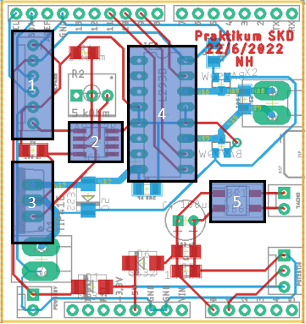
\includegraphics[width=\textwidth]{assets/konektor_pcb_1.png}};
			\begin{scope}[x={(img.south east)}, y={(img.north west)}]
				% Konektor (komponen 1--5 sudah ditandai pada gambar tata letak)
				\draw[konek] (0.82,0.60) rectangle (0.97,0.76); \node[koneklbl, anchor=east] at (0.82,0.68) {A};
				\draw[konek] (0.89,0.32) rectangle (0.97,0.43); \node[koneklbl, anchor=south] at (0.93,0.43) {B};
				\draw[konek] (0.89,0.08) rectangle (0.97,0.24); \node[koneklbl, anchor=east] at (0.89,0.16) {C};
				\draw[konek] (0.06,0.13) rectangle (0.20,0.27); \node[koneklbl, anchor=west] at (0.20,0.20) {D};
				\draw[konek] (0.06,0.02) rectangle (0.15,0.11); \node[koneklbl, anchor=west] at (0.15,0.065) {E};
			\end{scope}
		\end{tikzpicture}
	\end{minipage}\hfill
	\begin{minipage}{0.47\textwidth}
		\centering
		\begin{tikzpicture}
			\node[anchor=south west, inner sep=0] (img) {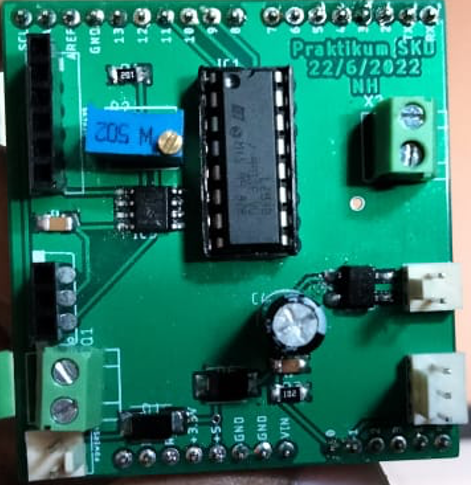
\includegraphics[width=\textwidth]{assets/konektor_pcb_2.png}};
			\begin{scope}[x={(img.south east)}, y={(img.north west)}]
				% Komponen
				\draw[komp] (0.05,0.60) rectangle (0.17,0.94); \node[komplbl] at (0.11,0.77) {1};
				\draw[komp] (0.24,0.51) rectangle (0.38,0.62); \node[komplbl] at (0.31,0.565) {2};
				\draw[komp] (0.05,0.29) rectangle (0.17,0.48); \node[komplbl] at (0.11,0.385) {3};
				\draw[komp] (0.41,0.47) rectangle (0.64,0.87); \node[komplbl] at (0.525,0.67) {4};
				\draw[komp] (0.70,0.36) rectangle (0.82,0.46); \node[komplbl] at (0.76,0.41) {5};
				% Konektor
				\draw[konek] (0.76,0.62) rectangle (0.92,0.81); \node[koneklbl, anchor=east] at (0.76,0.715) {A};
				\draw[konek] (0.85,0.34) rectangle (0.97,0.47); \node[koneklbl, anchor=south] at (0.91,0.47) {B};
				\draw[konek] (0.86,0.10) rectangle (0.98,0.27); \node[koneklbl, anchor=east] at (0.86,0.185) {C};
				\draw[konek] (0.08,0.12) rectangle (0.19,0.29); \node[koneklbl, anchor=west] at (0.19,0.205) {D};
				\draw[konek] (0.04,0.01) rectangle (0.19,0.11); \node[koneklbl, anchor=west] at (0.19,0.06) {E};
			\end{scope}
		\end{tikzpicture}
	\end{minipage}
	\caption{Posisi komponen dan konektor pada PCB \textit{shield}: tata letak PCB (kiri) dan foto PCB (kanan). Komponen: (1)~DAC MCP4725, (2)~OpAmp AD712, (3)~transistor TIP41C, (4)~L293D, (5)~penyearah MB6S. Konektor: (A)~motor, (B)~tachometer, (C)~potensiometer, (D)~catu daya 24~V, (E)~catu daya 5~V}
	\label{fig:konektor_pcb}
\end{figure}

\subsection{Akuisisi Data dan Pewaktuan Diskrit}

\subsubsection{Kuantisasi ADC}
ADC 10-bit Arduino UNO dengan tegangan referensi 5~V memiliki resolusi
\begin{equation}
	\Delta V = \frac{5~\text{V}}{1023} \approx 4{,}89~\text{mV per tingkat}.
	\label{eq:resolusi_adc}
\end{equation}
Program praktikum mengubah hasil pembacaan ADC $N$ menjadi persen agar sensor posisi dan kecepatan memiliki satuan yang seragam:
\begin{equation}
	y_{\%} = \frac{N}{1023} \times 100\%.
	\label{eq:adc_persen}
\end{equation}
Satu kali pembacaan \texttt{analogRead()} pada Arduino UNO membutuhkan waktu sekitar 0,1~ms. Program praktikum menyediakan dua cara akuisisi: pengambilan satu sampel (fungsi \texttt{sample\_...}) dan perataan beberapa sampel (fungsi \texttt{smooth\_...}). Perbandingan keduanya akan dianalisis pada Modul 1.

\subsubsection{Waktu Cacah}
Dalam kontrol diskrit, sensor dibaca dan aksi kontrol diperbarui setiap selang waktu tetap $T_s$ yang disebut \textbf{waktu cacah} (\textit{sampling time}). Sinyal kontinu $y(t)$ hanya diamati pada saat-saat $t = kT_s$, menghasilkan barisan
\begin{equation}
	y[k] = y(kT_s), \qquad k = 0, 1, 2, \ldots
	\label{eq:cacah}
\end{equation}
Agar model dan perhitungan kontrol diskrit berlaku, $T_s$ harus konsisten dari satu cacah ke cacah berikutnya. Ada dua cara umum untuk membuat jeda pada program Arduino:
\begin{enumerate}
	\item \textbf{Menggunakan \texttt{delay()}}. Program berhenti selama $T_d$, lalu menjalankan seluruh isi \texttt{loop()}. Periode satu putaran menjadi $T = T_d + T_{proses}$, dengan $T_{proses}$ adalah waktu eksekusi instruksi (pembacaan sensor, perhitungan, komunikasi serial). Karena $T_{proses}$ dapat berubah-ubah, periode tidak tetap. Selain itu, selama \texttt{delay()} program tidak dapat melakukan hal lain.
	\item \textbf{Menggunakan \texttt{millis()} (\textit{time sampling})}. Program terus berputar dan memeriksa apakah waktu yang berlalu sejak cacah terakhir sudah mencapai $T_s$:
	      \begin{lstlisting}[numbers=none]
Time = millis();
if (Time - LastTime >= TimeSampling) {
  DeltaTime = Time - LastTime;
  LastTime = Time;
  // akuisisi, perhitungan kontrol, dan aksi kontrol
}\end{lstlisting}
	      Selama $T_{proses} < T_s$, periode cacah akan tetap sama dengan $T_s$ dan program tetap dapat menjalankan tugas lain (misalnya menerima masukan serial) di luar blok \texttt{if}.
\end{enumerate}
Variabel yang menyimpan nilai \texttt{millis()} dideklarasikan sebagai \texttt{unsigned long} agar tidak terjadi luapan (\textit{overflow}) dalam waktu singkat.

\subsubsection{Komunikasi Serial}
Arduino UNO berkomunikasi dengan laptop melalui serial USB dengan \textit{baudrate} \textbf{115200} bit/s pada program praktikum. Pengaturan \textit{baudrate} pada \textit{Serial Monitor} harus sama; bila berbeda, data yang tampil akan berupa karakter acak. Pengiriman satu karakter membutuhkan sekitar 10 bit, sehingga pada 115200 bit/s satu karakter memerlukan sekitar 0,087~ms. Mencetak banyak data setiap cacah ikut menambah $T_{proses}$.

Masukan dari laptop dibaca oleh fungsi \texttt{serial()} (Lampiran~\ref{lamp:kode}, Kode~\ref{lst:serial}) dengan aturan sebagai berikut:
\begin{itemize}
	\item Teks dibaca hingga karakter \textit{newline} (\texttt{\textbackslash n}), lalu dikonversi menjadi bilangan bulat dengan \texttt{toInt()}.
	\item Nilai di atas 100 dibatasi menjadi 100, nilai di bawah $-100$ dibatasi menjadi $-100$.
	\item Pengaturan akhir baris pada \textit{Serial Monitor} sebaiknya \textbf{Newline}. Pengaturan lain menyebabkan fungsi menunggu hingga batas waktu (\textit{timeout}) sebelum memproses masukan.
\end{itemize}

\subsection{Struktur Program Praktikum}
Program praktikum disusun dalam beberapa \textit{tab} (file \texttt{.ino}) di dalam satu folder \textit{sketch}. Arduino IDE menggabungkan seluruh tab sesuai urutan nama file saat kompilasi, sehingga fungsi pada satu tab dapat dipanggil dari tab lain. Pembagian tab ditunjukkan pada Tabel~\ref{tab:struktur_program}.

\begin{table}[H]
	\centering
	\caption{Struktur program praktikum}
	\label{tab:struktur_program}
	\begin{tabularx}{\textwidth}{|l|X|l|}
		\hline
		\textbf{Tab}                 & \textbf{Isi}                                                                             & \textbf{Modul} \\
		\hline
		\sketch                      & Pengaturan umum, yaitu inisialisasi serial 115200 (\texttt{general\_setup()})            & 0--4           \\
		\prog{1\_sensor.ino}         & Definisi pin sensor, fungsi akuisisi posisi dan kecepatan (\texttt{sample}, \texttt{smooth}) & 0--4       \\
		\prog{2\_actuator.ino}       & Inisialisasi DAC dan pin arah, fungsi \texttt{run\_motor()}                              & 0--4           \\
		\prog{3\_serial.ino}         & Fungsi \texttt{serial()} untuk membaca masukan dari \textit{Serial Monitor}               & 0--4           \\
		\prog{4\_compensation.ino}   & Fungsi kompensasi \textit{deadzone}                                                      & 1--4           \\
		\prog{5\_control.ino}        & Fungsi perhitungan aksi kontrol                                                           & 2--4           \\
		\prog{6\_state\_space.ino}   & Model ruang keadaan, umpan balik keadaan, dan observer                                    & 4              \\
		\prog{9\_main.ino}           & Program utama: \texttt{setup()} dan \texttt{loop()}                                       & 0--4           \\
		\hline
	\end{tabularx}
\end{table}

Tab \prog{9\_main.ino} adalah satu-satunya tab yang berisi \texttt{setup()} dan \texttt{loop()}. Untuk setiap percobaan, praktikan cukup \textbf{mengganti isi tab \prog{9\_main.ino}} dengan program utama yang sesuai. Program utama contoh untuk Modul 0 ditunjukkan pada Tabel~\ref{tab:program_utama}.

\begin{table}[H]
	\centering
	\caption{Program utama contoh untuk Modul 0}
	\label{tab:program_utama}
	\begin{tabularx}{\textwidth}{|c|l|X|}
		\hline
		\textbf{No} & \textbf{File}                        & \textbf{Fungsi}                                                                                     \\
		\hline
		1           & \prog{1\_main\_akuisisi\_data}       & Membaca potensiometer dan tachometer dengan tiga cara: nilai ADC mentah, persen satu sampel, dan persen rata-rata 10 sampel \\
		2           & \prog{2\_main\_time}                 & Menambahkan waktu berjalan dan \texttt{DeltaTime} (lama satu putaran \texttt{loop()}) pada keluaran \\
		3           & \prog{3\_main\_delay}                & Menunjukkan pengaruh \texttt{delay()} terhadap periode putaran \texttt{loop()}                      \\
		4           & \prog{4\_main\_time\_sampling}       & Menunjukkan pencacahan waktu berbasis \texttt{millis()}                                              \\
		5           & \prog{5\_main\_motor}                & Menggerakkan motor menggunakan masukan dari \textit{Serial Monitor} sambil membaca kedua sensor     \\
		\hline
	\end{tabularx}
\end{table}

Fungsi \texttt{run\_motor()} (Kode~\ref{lst:actuator}) menerima masukan $-100$ hingga $100$~persen. Fungsi ini membatasi masukan pada rentang tersebut, mengatur arah melalui L293D, lalu mengirim besar tegangan ke DAC sesuai Persamaan~\eqref{eq:dac}. Bila arah masukan berbalik dari cacah sebelumnya, fungsi ini akan mengerem motor terlebih dahulu selama satu cacah.

% ===========================================================================
\section[Keselamatan Kerja dan SOP]{Keselamatan Kerja dan Prosedur Standar Operasional}
% ===========================================================================
\subsection{Keselamatan Kerja}
\begin{enumerate}
	\item Pastikan tangan dan meja kerja kering. Kit praktikum terhubung dengan listrik 220~V AC melalui power supply.
	\item Jangan membuka atau menyentuh terminal masukan AC pada power supply ketika kabel listrik terhubung.
	\item Jauhkan jari, rambut, kabel, dan benda lain dari roda gigi ketika motor berputar.
	\item Transistor TIP41C dan \textit{heat sink}-nya dapat menjadi panas. Jangan menyentuhnya segera setelah motor dijalankan dengan masukan besar.
	\item Laporkan kepada asisten apabila tercium bau hangus, terlihat asap, atau terdapat komponen yang terasa sangat panas, lalu segera cabut kabel listrik.
\end{enumerate}

\subsection{Pencegahan Kerusakan Kit}
\begin{enumerate}
	\item \textbf{Jangan mengubah pemasangan kabel dan komponen ketika kit sedang dialiri listrik.} Cabut kabel listrik 220~V dan kabel USB terlebih dahulu.
	\item Pastikan orientasi konektor dan komponen lepasan (MCP4725, TIP41C, L293D) benar sebelum kit dinyalakan. Pemasangan terbalik dapat merusak komponen secara permanen.
	\item Hindari hubung singkat. Jangan meletakkan benda logam, kabel jumper lepas, atau obeng di atas PCB.
	\item \textbf{Uji program baru tanpa daya motor.} Sebelum menjalankan program yang baru diunggah atau dimodifikasi, pastikan program berjalan sesuai keinginan dengan mengamati \textit{Serial Monitor} ketika kabel listrik 220~V belum terhubung atau ketika transistor TIP41C dilepas. Dengan demikian motor tidak akan berputar walaupun program memberikan masukan.
	\item Panggil \texttt{run\_motor()} hanya di dalam blok waktu cacah. Memanggil fungsi ini terus-menerus di dalam \texttt{loop()} tanpa waktu cacah akan membebani komunikasi I$^2$C dan memperbesar kemungkinan kerusakan kit.
	\item Jangan mengubah masukan motor dari positif langsung ke negatif (atau sebaliknya). Berikan masukan nol terlebih dahulu dan tunggu motor berhenti.
	\item Jangan menahan atau menghentikan poros motor dengan tangan ketika motor diberi masukan.
	\item Jangan memutar trimpot penguatan OpAmp kecuali diminta dalam prosedur.
\end{enumerate}

\peringatan{Kit praktikum sangat rentan rusak bila \texttt{loop()} program tidak bekerja sesuai keinginan. Selalu verifikasi program tanpa daya motor terlebih dahulu.}

\subsection{Urutan Menyalakan dan Mematikan Kit}
\textbf{Menyalakan kit:}
\begin{enumerate}
	\item Periksa kelengkapan dan pemasangan konektor serta komponen lepasan.
	\item Hubungkan Arduino UNO ke laptop menggunakan kabel USB.
	\item Unggah program dan verifikasi melalui \textit{Serial Monitor} (tanpa daya motor).
	\item Hubungkan kabel listrik power supply ke stop kontak 220~V. Lampu indikator power supply akan menyala.
\end{enumerate}
\textbf{Mematikan kit:}
\begin{enumerate}
	\item Kirim masukan nol dan tunggu hingga motor berhenti.
	\item Cabut kabel listrik 220~V dari stop kontak.
	\item Cabut kabel USB dari laptop.
	\item Rapikan kabel dan kembalikan kit dalam kondisi lengkap.
\end{enumerate}

% ===========================================================================
\section{Prosedur Praktikum}
% ===========================================================================
Prosedur Modul 0 terdiri atas persiapan dan enam percobaan. Catat seluruh hasil pengamatan pada tabel yang disediakan dan simpan data dari \textit{Serial Monitor} ke dalam \textit{spreadsheet} untuk dilampirkan pada laporan.

\subsection{Persiapan Sebelum Praktikum}
Langkah-langkah berikut dikerjakan sebelum jadwal praktikum:
\begin{enumerate}
	\item Unduh dan instal Arduino IDE.
	\item Instal \textit{library} \textbf{Adafruit MCP4725} melalui menu \textit{Tools} $\rightarrow$ \textit{Manage Libraries}. \textit{Library} pendukung yang diminta (misalnya Adafruit BusIO) ikut diinstal.
	\item Unduh program praktikum dari repositori, lalu buka \sketch. Pastikan seluruh tab pada Tabel~\ref{tab:struktur_program} muncul.
	\item Pilih \textit{board} \textbf{Arduino Uno} pada menu \textit{Tools} $\rightarrow$ \textit{Board}, lalu lakukan \textit{Verify/Compile}. Kompilasi harus berhasil tanpa galat.
	\item Siapkan MATLAB, baik versi desktop maupun MATLAB Online.
	\item Baca seluruh modul ini, terutama Bagian Keselamatan Kerja dan SOP.
\end{enumerate}

\subsection{Percobaan 1: Identifikasi Komponen Kit}
Percobaan ini dilakukan \textbf{tanpa} menghubungkan kit ke listrik maupun laptop.
\begin{enumerate}
	\item Catat nomor kit praktikum yang digunakan.
	\item Identifikasi setiap komponen pada kit dengan bantuan Gambar~\ref{fig:kit_praktikum} hingga Gambar~\ref{fig:konektor_pcb}.
	\item Periksa pemasangan setiap konektor dan komponen lepasan menggunakan label pada Gambar~\ref{fig:konektor_pcb}, lalu lengkapi Tabel~\ref{tab:p1_komponen}. Perhatikan orientasi transistor TIP41C dan takik (\textit{notch}) IC L293D pada soketnya.
	\item Putar roda gigi potensiometer secara perlahan dengan tangan dan amati bahwa roda gigi motor ikut berputar. Hitung berapa putaran poros motor untuk satu putaran potensiometer, lalu bandingkan dengan Persamaan~\eqref{eq:rasio_gigi}.
\end{enumerate}

\begin{table}[H]
	\centering
	\caption{Pemeriksaan komponen kit praktikum (Nomor kit: \underline{\hspace{1.5cm}})}
	\label{tab:p1_komponen}
	\begin{tabularx}{\textwidth}{|c|X|c|X|}
		\hline
		\textbf{No} & \textbf{Komponen / Konektor}    & \textbf{Kondisi (\checkmark/\texttimes)} & \textbf{Keterangan} \\
		\hline
		1           & (A) Konektor motor (X2)         &                    &                     \\
		2           & (B) Konektor tachometer (TACHO) &                    &                     \\
		3           & (C) Konektor potensiometer (POTENTIO) &              &                     \\
		4           & (D) Konektor catu daya 24 V     &                    &                     \\
		5           & (E) Konektor catu daya 5 V (POWER5V) &               &                     \\
		6           & (1) Modul DAC MCP4725           &                    &                     \\
		7           & (3) Transistor TIP41C + heat sink &                  &                     \\
		8           & (4) IC L293D                    &                    &                     \\
		9           & Roda gigi motor dan potensiometer &                  &                     \\
		10          & Kabel USB dan kabel listrik     &                    &                     \\
		\hline
	\end{tabularx}
\end{table}

\subsection{Percobaan 2: Pemeriksaan Catu Daya}
\begin{enumerate}
	\item Lepaskan konektor catu daya 24~V dan 5~V dari PCB.
	\item Hubungkan kabel listrik power supply ke stop kontak 220~V. Pastikan lampu indikator menyala.
	\item Ukur tegangan keluaran power supply menggunakan multimeter pada mode tegangan DC.
	\item Ukur tegangan keluaran konverter DC--DC.
	\item Cabut kabel listrik, lalu pasang kembali kedua konektor catu daya ke PCB.
	\item Lengkapi Tabel~\ref{tab:p2_catu_daya}. Laporkan kepada asisten bila tegangan menyimpang lebih dari 5\% dari nilai nominal.
\end{enumerate}

\begin{table}[H]
	\centering
	\caption{Hasil pemeriksaan catu daya}
	\label{tab:p2_catu_daya}
	\begin{tabular}{|l|c|c|c|}
		\hline
		\textbf{Sumber}       & \textbf{Nominal (V)} & \textbf{Terukur (V)} & \textbf{Penyimpangan (\%)} \\
		\hline
		Power supply AC--DC   & 24                   &                      &                            \\
		Konverter DC--DC      & 5                    &                      &                            \\
		\hline
	\end{tabular}
\end{table}

\subsection{Percobaan 3: Unggah Program dan Akuisisi Data Sensor}
Percobaan ini dilakukan dengan kabel USB terhubung, tetapi \textbf{kabel listrik 220~V tidak terhubung}.
\begin{enumerate}
	\item Hubungkan Arduino UNO ke laptop dengan kabel USB.
	\item Pilih port Arduino pada menu \textit{Tools} $\rightarrow$ \textit{Port}. Pada Windows, port dapat dicek pada \textit{Device Manager} (misalnya \texttt{COM3}); pada macOS/Linux, port bernama \texttt{/dev/cu.usbmodem...} atau \texttt{/dev/ttyACM...}.
	\item Ganti isi tab \prog{9\_main.ino} dengan \prog{1\_main\_akuisisi\_data}, lalu unggah program.
	\item Buka \textit{Serial Monitor} dan atur \textit{baudrate} menjadi 115200. Amati enam kolom data: posisi dan kecepatan dalam nilai ADC mentah, persen satu sampel, dan persen rata-rata.
	\item Putar roda gigi potensiometer dengan tangan secara perlahan hingga bacaan posisi berada di sekitar 25\%, 50\%, dan 75\%. Pada setiap posisi, catat nilai pada Tabel~\ref{tab:p3_akuisisi}.
	\item Periksa hubungan nilai ADC mentah dan nilai persen menggunakan Persamaan~\eqref{eq:adc_persen}.
	\item Tutup \textit{Serial Monitor}, buka \textit{Serial Plotter}, lalu putar potensiometer dan amati grafiknya. Simpan tangkapan layar.
	\item Laporkan kepada asisten bila bacaan potensiometer tidak berubah ketika diputar atau berfluktuasi lebih dari 2\% ketika diam.
\end{enumerate}

\begin{table}[H]
	\centering
	\caption{Hasil akuisisi data sensor posisi}
	\label{tab:p3_akuisisi}
	\begin{tabularx}{\textwidth}{|C|C|C|C|C|}
		\hline
		\textbf{Target posisi} & \textbf{ADC mentah} & \textbf{Persen (sampel)} & \textbf{Persen (rata-rata)} & \textbf{Persen dari Pers.~\eqref{eq:adc_persen}} \\
		\hline
		$\approx$25\%        &                     &                          &                             &                            \\
		$\approx$50\%        &                     &                          &                             &                            \\
		$\approx$75\%        &                     &                          &                             &                            \\
		\hline
	\end{tabularx}
\end{table}

\subsection{Percobaan 4: Waktu Eksekusi, \texttt{delay()}, dan Waktu Cacah}
Kabel listrik 220~V tetap tidak terhubung.
\begin{enumerate}
	\item Ganti tab \prog{9\_main.ino} dengan \prog{2\_main\_time}, lalu unggah. Kolom \texttt{Delta} menunjukkan lama satu putaran \texttt{loop()} dalam milidetik.
	\item Salin minimal 20 baris data dari \textit{Serial Monitor} ke \textit{spreadsheet}, lalu hitung nilai minimum, maksimum, dan rata-rata \texttt{Delta}. Hasil ini adalah waktu proses $T_{proses}$ program akuisisi.
	\item Ganti tab \prog{9\_main.ino} dengan \prog{3\_main\_delay}. Untuk nilai \texttt{TimeSampling} sebesar 10, 50, dan 100~ms (nilai \texttt{Delay} mengikuti \texttt{TimeSampling}), unggah program dan catat statistik \texttt{Delta}.
	\item Ganti tab \prog{9\_main.ino} dengan \prog{4\_main\_time\_sampling}. Ulangi langkah 3 untuk nilai \texttt{TimeSampling} yang sama.
	\item Lengkapi Tabel~\ref{tab:p4_waktu}.
\end{enumerate}

\begin{table}[H]
	\centering
	\caption{Perbandingan periode putaran \texttt{loop()} (dalam milidetik)}
	\label{tab:p4_waktu}
	\begin{tabularx}{\textwidth}{|l|c|C|C|C|}
		\hline
		\textbf{Program}                    & \textbf{$T_s$ (ms)} & \textbf{Delta min} & \textbf{Delta maks} & \textbf{Delta rata-rata} \\
		\hline
		\prog{2\_main\_time}               & --                    &                    &                     &                          \\
		\hline
		\prog{3\_main\_delay} & 10                &                    &                     &                          \\
		                                   & 50                    &                    &                     &                          \\
		                                   & 100                   &                    &                     &                          \\
		\hline
		\prog{4\_main\_time\_sampling}     & 10                    &                    &                     &                          \\
		                                   & 50                    &                    &                     &                          \\
		                                   & 100                   &                    &                     &                          \\
		\hline
	\end{tabularx}
\end{table}

\subsection{Percobaan 5: Menggerakkan Motor dan Masukan Serial}
\textbf{Bagian A -- verifikasi program tanpa daya motor.} Kabel listrik 220~V \textbf{belum} terhubung.
\begin{enumerate}
	\item Ganti tab \prog{9\_main.ino} dengan \prog{5\_main\_motor}, lalu unggah. Atur akhir baris \textit{Serial Monitor} menjadi \textbf{Newline}.
	\item Kirim masukan sesuai Tabel~\ref{tab:p5_serial} satu per satu. Untuk setiap masukan, catat nilai kolom \texttt{Input} dan \texttt{Motor} yang tampil. Motor tidak akan berputar karena belum mendapat daya.
	\item Ubah pengaturan akhir baris menjadi \textbf{No line ending}, kirim masukan \texttt{20}, lalu amati kolom \texttt{Delta} pada saat masukan diterima. Kembalikan pengaturan ke \textbf{Newline} dan kirim \texttt{0}.
\end{enumerate}

\begin{table}[H]
	\centering
	\caption{Pengujian masukan serial (tanpa daya motor)}
	\label{tab:p5_serial}
	\begin{tabular}{|c|l|c|c|l|}
		\hline
		\textbf{No} & \textbf{Masukan dikirim} & \textbf{Kolom Input} & \textbf{Kolom Motor} & \textbf{Keterangan} \\
		\hline
		1           & \texttt{30}              &                      &                      &                     \\
		2           & \texttt{-30}             &                      &                      &                     \\
		3           & \texttt{150}             &                      &                      &                     \\
		4           & \texttt{-150}            &                      &                      &                     \\
		5           & \texttt{25.7}            &                      &                      &                     \\
		6           & \texttt{abc}             &                      &                      &                     \\
		7           & \texttt{0}               &                      &                      &                     \\
		\hline
	\end{tabular}
\end{table}

\textbf{Bagian B -- menggerakkan motor.} Setelah program terverifikasi:
\begin{enumerate}
	\item Pastikan masukan terakhir adalah \texttt{0}, lalu hubungkan kabel listrik 220~V.
	\item Kirim masukan \texttt{30}. Amati arah putar poros motor (dilihat dari depan, sisi roda gigi), arah perubahan bacaan potensiometer (naik atau turun), dan bacaan tachometer.
	\item Kirim \texttt{0} dan tunggu motor berhenti.
	\item Kirim masukan \texttt{-30} dan lakukan pengamatan yang sama.
	\item Kirim \texttt{0} dan tunggu motor berhenti.
	\item Ulangi untuk masukan \texttt{60} dan \texttt{-60}, dengan masukan \texttt{0} di antara keduanya.
	\item Lengkapi Tabel~\ref{tab:p5_motor}. Simpan data \textit{Serial Monitor} dan tangkapan layar \textit{Serial Plotter} untuk satu masukan positif dan satu masukan negatif.
	\item Matikan kit sesuai urutan pada SOP.
\end{enumerate}

\begin{table}[H]
	\centering
	\caption{Pengamatan arah putar dan respons sensor}
	\label{tab:p5_motor}
	\begin{tabularx}{\textwidth}{|C|C|C|C|}
		\hline
		\textbf{Masukan (\%)} & \textbf{Arah putar motor} & \textbf{Bacaan posisi (naik/turun)} & \textbf{Bacaan kecepatan (\%)} \\
		\hline
		30                    &                           &                                     &                                \\
		$-30$                 &                           &                                     &                                \\
		60                    &                           &                                     &                                \\
		$-60$                 &                           &                                     &                                \\
		\hline
	\end{tabularx}
\end{table}

\subsection{Percobaan 6: Verifikasi Lingkungan MATLAB}
\begin{enumerate}
	\item Buka MATLAB atau MATLAB Online.
	\item Unggah atau buka folder program simulasi dari repositori praktikum.
	\item Jalankan program simulasi utama dan pastikan grafik respons sistem muncul tanpa galat.
	\item Simpan tangkapan layar hasil simulasi. Program ini akan digunakan mulai Modul 1 dan Modul 2.
\end{enumerate}

% ===========================================================================
\section{Laporan dan Pertanyaan}
% ===========================================================================
\subsection{Ketentuan Laporan}
% TODO: sesuaikan platform dan tenggat pengumpulan
Laporan Modul 0 dikumpulkan per kelompok melalui Edunex paling lambat satu minggu setelah praktikum. Laporan berupa file \texttt{.pdf} yang dilampiri \textit{spreadsheet} data dan program utama yang dimodifikasi (bila ada), digabung dalam satu file \texttt{.zip}. Laporan minimal berisi:
\begin{enumerate}
	\item Tabel~\ref{tab:p1_komponen} hingga Tabel~\ref{tab:p5_motor} yang telah dilengkapi beserta tangkapan layar yang diminta.
	\item Jawaban atas pertanyaan pada Bagian~\ref{sec:pertanyaan}.
	\item Tabel kontribusi anggota kelompok (Tabel~\ref{tab:kontribusi}).
\end{enumerate}

\begin{table}[H]
	\centering
	\caption{Kontribusi anggota kelompok}
	\label{tab:kontribusi}
	\begin{tabularx}{\textwidth}{|c|c|l|X|}
		\hline
		\textbf{No} & \textbf{NIM} & \textbf{Nama Lengkap} & \textbf{Kontribusi} \\
		\hline
		1           &              &                       &                     \\
		2           &              &                       &                     \\
		3           &              &                       &                     \\
		4           &              &                       &                     \\
		5           &              &                       &                     \\
		\hline
	\end{tabularx}
\end{table}

\subsection{Pertanyaan}
\label{sec:pertanyaan}
\begin{enumerate}
	\item Gambarkan diagram blok kit praktikum secara lebih rinci daripada Gambar~\ref{fig:skd_arsitektur}, mulai dari masukan \textit{Serial Monitor} hingga keluaran sensor yang diterima Arduino. Pada setiap panah, tuliskan jenis sinyal (digital/analog), rentang nilainya, dan satuannya.
	\item Berapa resolusi pengukuran posisi dalam persen, dalam derajat poros potensiometer, dan dalam derajat poros motor? Gunakan Persamaan~\eqref{eq:rasio_gigi} dan \eqref{eq:resolusi_adc}, serta asumsikan rentang 0--100\% setara dengan satu putaran potensiometer.
	\item Berapa resolusi tegangan DAC MCP4725? Berapa perubahan masukan motor terkecil (dalam persen) yang dapat dihasilkan oleh DAC?
	\item Berdasarkan Tabel~\ref{tab:p4_waktu}, bandingkan periode putaran \texttt{loop()} pada program \texttt{delay()} dan program \textit{time sampling}. Program mana yang lebih sesuai untuk sistem kontrol diskrit? Jelaskan.
	\item Berdasarkan Tabel~\ref{tab:p5_serial} dan kode fungsi \texttt{serial()}, jelaskan perlakuan program terhadap masukan di luar rentang, masukan pecahan, dan masukan bukan angka. Mengapa pengaturan \textit{No line ending} menghasilkan \texttt{Delta} yang jauh lebih besar?
	\item Jelaskan hubungan antara tanda masukan motor, arah putar motor, dan arah perubahan bacaan potensiometer berdasarkan Tabel~\ref{tab:p5_motor}.
	\item Perhatikan fungsi \texttt{run\_motor()}. Apa tujuan baris berikut?
	      \begin{center}\texttt{if (Direction * LastDirection < 0) Direction = fast\_break();}\end{center}
	      Apa yang dapat terjadi pada rangkaian driver bila baris ini tidak ada?
	\item Perhatikan rangkaian pengkondisi sinyal tachometer (Gambar~\ref{fig:rangkaian_tacho}) dan Persamaan~\eqref{eq:tau_filter}. Bandingkan konstanta waktu filter dengan waktu cacah 100~ms pada program \prog{5\_main\_motor}. Bagaimana filter ini dapat memengaruhi hasil identifikasi dinamika motor yang akan dilakukan pada Modul~1?
	\item Sebutkan minimal tiga langkah SOP yang paling penting menurut kelompok Anda, beserta risiko yang dicegah oleh masing-masing langkah.
\end{enumerate}

% ===========================================================================
\section{Penutup}
% ===========================================================================
Dengan menyelesaikan Modul 0, kit praktikum dan perangkat lunak telah siap digunakan, dan praktikan telah memahami komponen, struktur program, serta prosedur pengoperasian kit. Pada Modul 1, praktikan akan menggunakan kemampuan ini untuk mengamati hubungan masukan dan keluaran motor, merancang kompensasi \textit{deadzone}, menentukan waktu cacah, dan mengidentifikasi model kecepatan motor DC. Simpan program dan data Modul 0 karena akan digunakan kembali.

% ===========================================================================
\appendix
\section{Kode Program Pendukung}
\label{lamp:kode}
% ===========================================================================

\begin{lstlisting}[caption={Tab \texttt{1\_sensor.ino}},label={lst:sensor}]
#define PinTachometer A0
#define PinPotensiometer A1

int MaxTachometer = 1023;

void sensor_setup() {
  pinMode(PinTachometer, INPUT);
  pinMode(PinPotensiometer, INPUT);
}

float sample_velocity_percentage() {
  return (float) analogRead(PinTachometer) * 100 / MaxTachometer;
}

float sample_position_percentage() {
  return (float) analogRead(PinPotensiometer) * 100 / 1023;
}

float smooth_pin(int Pin, byte SizeRead) {
  unsigned int TotalRead = 0;
  for (byte i = 0; i < SizeRead; i++) {
    TotalRead += analogRead(Pin);
  }
  return (float) TotalRead / SizeRead;
}

float smooth_velocity_percentage() {
  return smooth_pin(PinTachometer, 10) * 100 / MaxTachometer;
}

float smooth_position_percentage() {
  return smooth_pin(PinPotensiometer, 10) * 100 / 1023;
}
\end{lstlisting}

\begin{lstlisting}[caption={Tab \texttt{2\_actuator.ino}},label={lst:actuator}]
#include <Adafruit_MCP4725.h>

#define PinEn 11
#define PinIn1 10
#define PinIn2 9

int Direction, LastDirection = 0;
Adafruit_MCP4725 DAC;

void actuator_setup() {
  DAC.begin(0x60);
  pinMode(PinEn, OUTPUT);
  pinMode(PinIn1, OUTPUT);
  pinMode(PinIn2, OUTPUT);
  digitalWrite(PinEn, HIGH);
  digitalWrite(PinIn1, LOW);
  digitalWrite(PinIn2, LOW);
}

int clock_wise() {
  digitalWrite(PinIn1, HIGH);
  digitalWrite(PinIn2, LOW);
  return 1;
}

int counter_clock_wise() {
  digitalWrite(PinIn2, HIGH);
  digitalWrite(PinIn1, LOW);
  return -1;
}

int fast_break() {
  digitalWrite(PinIn1, LOW);
  digitalWrite(PinIn2, LOW);
  return 0;
}

float percentage_limit(float Percent) {
  if (Percent > 100.0) return 100.0;
  else if (Percent < -100.0) return -100.0;
  else return Percent;
}

void set_voltage(int Sign, float Percent) {
  uint32_t InputMCP = Sign * 4095 * Percent / 100;
  DAC.setVoltage(InputMCP, false);
}

float run_motor(float InputPercentage) {
  InputPercentage = percentage_limit(InputPercentage);
  if (InputPercentage > 0.0) Direction = clock_wise();
  else if (InputPercentage < 0.0) Direction = counter_clock_wise();
  else Direction = fast_break();
  if (Direction * LastDirection < 0) Direction = fast_break();
  set_voltage(Direction, InputPercentage);
  LastDirection = Direction;
  return (float) Direction * Direction * InputPercentage;
}
\end{lstlisting}

\begin{lstlisting}[caption={Tab \texttt{3\_serial.ino}},label={lst:serial}]
int serial(int SerialRead) {
  if (Serial.available() > 0) {
    String StringSerial = Serial.readStringUntil('\n');
    SerialRead = StringSerial.toInt();
    if (SerialRead > 100) return 100;
    else if (SerialRead < -100) return -100;
  }
  return SerialRead;
}
\end{lstlisting}

\begin{lstlisting}[caption={Program utama \texttt{5\_main\_motor}},label={lst:main_motor}]
unsigned long Time, StartTime, LastTime;
unsigned int TimeSampling = 100, DeltaTime;
int InputSerial = 0;
float Motor = 0.0;
float Poten1, Poten2, Tacho1, Tacho2;

void setup() {
  general_setup();
  sensor_setup();
  actuator_setup();
  print_header();
  StartTime = millis();
  LastTime = StartTime;
}

void loop() {
  InputSerial = serial(InputSerial);
  Time = millis();
  if (Time - LastTime >= TimeSampling) {
    DeltaTime = Time - LastTime;
    LastTime = Time;
    Motor = run_motor((float) InputSerial);
    Poten1 = sample_position_percentage();
    Poten2 = smooth_position_percentage();
    Tacho1 = sample_velocity_percentage();
    Tacho2 = smooth_velocity_percentage();
    Serial.print(Time - StartTime - TimeSampling);
    Serial.print("\t");
    Serial.print(DeltaTime);
    Serial.print("\t");
    Serial.print(InputSerial);
    Serial.print("\t");
    Serial.print(Motor);
    Serial.print("\t");
    Serial.print(Poten1);
    Serial.print("\t");
    Serial.print(Poten2);
    Serial.print("\t");
    Serial.print(Tacho1);
    Serial.print("\t");
    Serial.println(Tacho2);
  }
}

void print_header() {
  Serial.println("Time\tDelta\tInput\tMotor\tPos 1\tPos 2\tKec 1\tKec 2");
}
\end{lstlisting}

\end{document}
